% !TEX root = Tesi.tex
\chead{}
\chapter{The combined approach}

\section{The IFML language}

The Interaction Flow Modeling Language (IFML)\cite{IFML-1, IFML-2} is designed for describing and controlling the behavior of front-end software applications, it brings several advantages to the development process such as promoting the separation of concerns between roles and increasing the overall understanding of the product for non-technical stakeholders. To achieve so IFML supports formal specification for interface composition, user interaction and event management independently of the implementation platform and it was adopted as a standard by the Object Management Group (OMG) in March 2013.

An IFML model supports the following design specifications: 

\begin{itemize}
  \item \textbf{The view structure} describes \textit{ViewContainers}, their nesting relationships, their visibility and their reachability.
  
  \item \textbf{The view content} manages \textit{ViewComponents}, i.e., content and data entry elements contained within ViewContainers.
  
  \item \textbf{The events} defines the \textit{Events} that may affect the state of the user interface. \textit{Events} can be produced by the user’s interaction, by the application, or by an external system; 

  \item \textbf{The event transition} indicates the effect of an Event on the user interface. 

  \item \textbf{The parameter binding} illustrates the input-output dependencies between \textit{ViewComponents} and between \textit{ViewComponents} and \textit{Actions}. 

  \item \textbf{The actions} triggered by the user’s events. The effect of an \textit{Event} is represented by an \textit{InteractionFlow} connection, which connects the event to the \textit{ViewContainer} or \textit{ViewComponent} affected by the \textit{Event}. The \textit{InteractionFlow} expresses a change of state of the user interface: the occurrence of the event triggers a change in the state that produces a transition in the user interface.

\end{itemize} 

\vspace{0.5cm}
\begin{figure}[htbp]
  \centering
    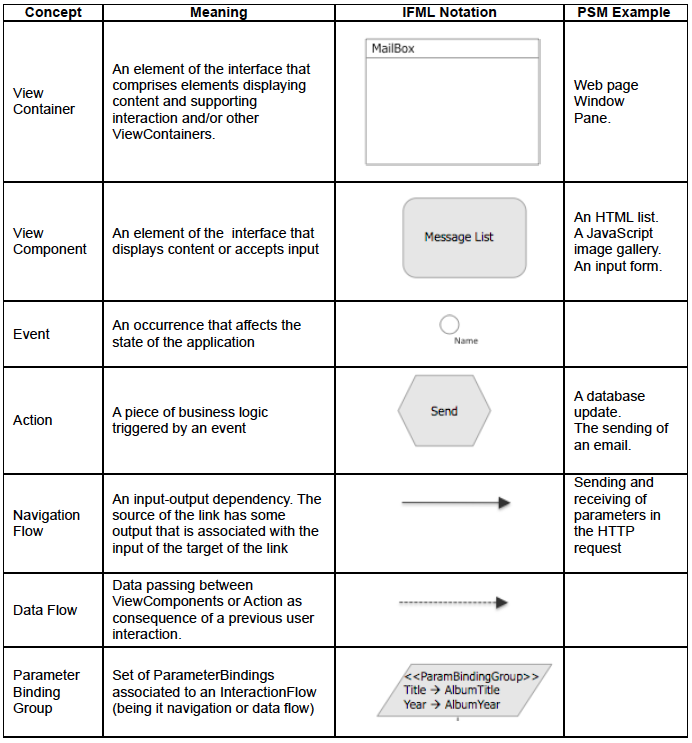
\includegraphics[height=10cm]{images/ifml.jpg}
  \caption{Main IFML concepts and notations.}
  \label{fig:ifml}
\end{figure}
\vspace{0.5cm}

\section{Representing and modeling user behaviours}

Lorem ipsum dolor sit amet, consectetur adipisici elit, sed eiusmod tempor incidunt ut labore et dolore magna aliqua.
Ut enim ad minim veniam, quis nostrud exercitation ullamco laboris nisi ut aliquid ex ea commodi consequat. Quis aute iure reprehenderit in voluptate velit esse cillum dolore eu fugiat nulla pariatur. Excepteur sint obcaecat cupiditat non proident, sunt in culpa qui officia deserunt
mollit anim id est laborumLorem ipsum dolor sit amet, consectetur adipisici elit, sed eiusmod tempor incidunt ut labore et dolore magna aliqua. Ut enim ad minim veniam, quis nostrud exercitation ullamco laboris nisi ut aliquid ex ea commodi consequat. Quis aute iure reprehenderit in voluptate velit esse cillum dolore eu fugiat nulla pariatur. Excepteur sint obcaecat cupiditat non proident, sunt in culpa qui officia deserunt mollit anim id est laborumLorem ipsum dolor sit amet, consectetur adipisici elit, sed eiusmod tempor incidunt ut labore et dolore magna aliqua. Ut enim ad minim veniam, quis nostrud exercitation ullamco laboris nisi ut aliquid ex ea commodi consequat. Quis aute iure reprehenderit in voluptate velit esse cillum dolore eu fugiat nulla pariatur. Excepteur sint obcaecat cupiditat non proident, sunt in culpa qui officia deserunt mollit anim id est laborumLorem ipsum dolor sit amet, consectetur adipisici elit, sed eiusmod tempor incidunt ut labore et dolore magna aliqua. Ut enim ad minim veniam, quis nostrud exercitation ullamco laboris nisi ut aliquid ex ea commodi consequat. Quis aute iure reprehenderit in voluptate velit esse cillum dolore eu fugiat nulla pariatur. Excepteur sint obcaecat cupiditat non proident, sunt in culpa qui officia deserunt mollit anim id est laborumLorem ipsum dolor sit amet, consectetur adipisici elit, sed eiusmod tempor incidunt ut labore et dolore magna aliqua. Ut enim ad minim veniam, quis nostrud exercitation ullamco laboris nisi ut aliquid ex ea commodi consequat.
Lorem ipsum dolor sit amet, consectetur adipisici elit, sed eiusmod tempor incidunt ut labore et dolore magna aliqua. Ut enim ad minim veniam, quis nostrud exercitation ullamco laboris nisi ut aliquid ex ea commodi consequat. Quis aute iure reprehenderit in voluptate velit esse cillum dolore eu

\section{Pattern recognition}



